\subsection{Conformational changes}
In this section the conformation of FAK bound to \pip{} containing membrane (FAK-MEM) is compared to the observations from \autoref{sec:fak_sol} (FAK-SOL). For this purpose the simulation data of setup 4 was used with the condition, that other FAK molecules are more than $2\,\si{\nano\metre}$ away (0 neighbours). The contact map is based on the same dataset, which was used in \autoref{forceana:intramolec}.\\
\\
Analogously to \autoref{sec:fak_sol} the distribution of the COM distances is presented in \autoref{mem:comdist} as an hexagonal binning plot. Again two spots can be identified, which show a large number of encounters. However these spots are much more smeared out than obtained in FAK-SOL. In addition larger values of $d_\text{F2-C}$ disappear. This is expected, as the kinase is also bound to the membrane, resulting in less deviations in the lower part of the protein. Also the contact area of the interface, which can be found in \autoref{mem:contactarea}, indicates a closure of the protein. \\
\\
In contrast the linker region containing the autophosphorylation site \acid{Y}{397} seems to be released from the two domains. On the one hand the mean distance to residues of the domain increases by up to $0.67\,\si{\nano\metre}$ (\acid{S}{74} and \acid{T}{394}), on the other hand the RMSF values are increasing as well, which indicates a more flexible region.\\
\\
The obtained results are consistent with previous observations. \pip does not induce the dissociation of the FERM domain and the kinase, but it enhances autophosphorylation. Later can not be simulated in MD simulation, but the changes in the linker region support this assumption.
%
%
%
\begin{figure}
	\subcaptionbox{Two dimensional histogram of $d_\text{F1-N}$ and $d_\text{F2-C}$\label{mem:comdist}}[0.46\textwidth]{
		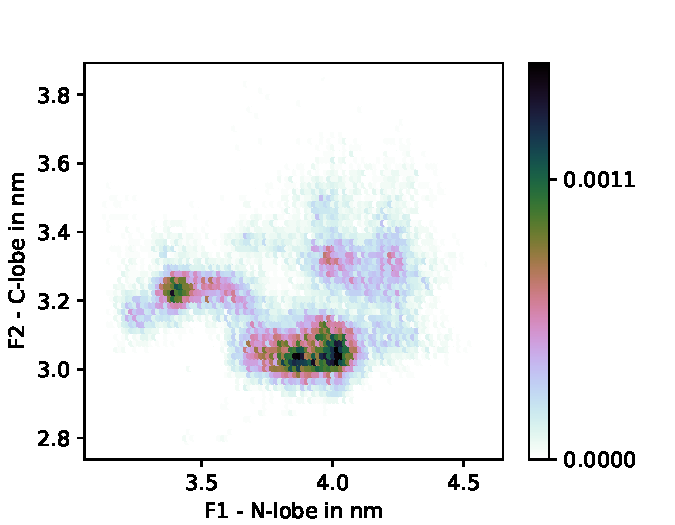
\includegraphics[height=5cm]{figures/results/membr_f1f2}
	}\hfill%
	\subcaptionbox{Contactarea of FERM-kinase interface\label{mem:contactarea}}[0.49\textwidth]{
		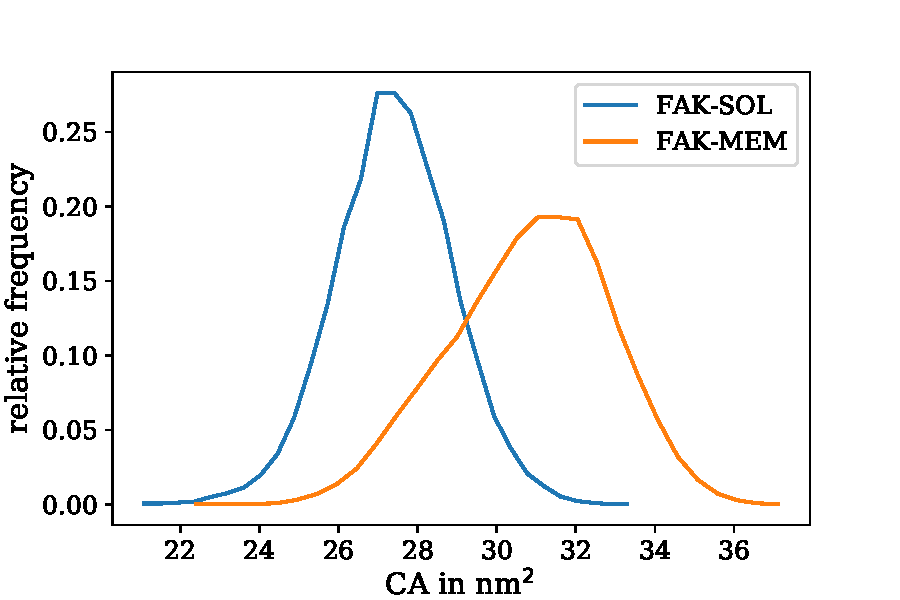
\includegraphics[height=5cm]{figures/results/ca_sol_mem}
	}%
	\phantomsubcaption
\end{figure}
%
%
%
% TODO: show contact map?
